\chapter{السلاسل المحرفيّة (\textenglish{Strings})}

السلاسل المحرفيّة هي اسم صحيح
\textit{برمجيّا}
لتسمية \dots النصّ، ببساطة !\\
السلسلة المحرفيّة هي إذن نصّ يمكننا حفظه على شكل متغيّر في الذاكرة. بهذه الطريقة يمكننا تخزين اسم المستخدم.

كنت قد قلت من قبل أن الحاسوب لا يفهم إلا الأعداد، فما هو السحر الذي يفعله المبرمجون للتعامل مع النصوص ؟ إنّهم ماكرون، سوف ترى !

\section{النوع \texttt{char}}

في هذا الفصل سنعطي أهمية خاصة للنوع
\InlineCode{char}.
إن كنت تتذكّر جيداً فهذا النوع يسمح بخزين الأعداد المحصورة بين
$-127$
و
$128$.

\begin{information}
  النوع
\InlineCode{char}
 يسمح بتخزين الأعداد، لكننا غالبا لا نستخدمه في لغة الـ\textenglish{C}
من أجل ذلك.
عادة، حتّى لو كان العدد صغيرا، فإنّنا نخزنه في
\InlineCode{int}.
بالطبع، هذا سيأخذ  شيئا أكبر من الذاكرة، لكن في هذه الأيّام، ليست الذاكرة ما ينقص الحواسيب فعلا.
\end{information}

إذا فالنوع
\InlineCode{char}
مستعمل لتخزين \dots "حرف" ! احذر، لقد قلت :
\underline{حرف واحد}.

و لأنّ الذاكرة لا يمكنها تخزين شيء سوى الأعداد، فلقد تمّ اختراع جدول يقوم بالتحويل بين الحروف و الأعداد. هذا الجدول يخبرنا مثلا أنّ العدد 65 مكافئ للحرف
\textenglish{A}.

لغة
\textenglish{C}
تسمح لنا بالقيام بالتحويل بين الحرف و العدد الموافق له. للحصول على العدد الموافق لحرف، يكفي كتابته بين علامتي تنصيص، هكذا :
\InlineCode{'A'}.
عند الترجمة، سيتم استبدال
\InlineCode{'A'}
بالقيمة الموافقة.

فلنجرّب :

\begin{Csource}
int main(int argc, char *argv[])
{
	char letter = 'A';
	printf("%d\n", letter );
	return 0;
}
\end{Csource}

نعلم إذن أن الحرف
\textenglish{A}
يمثل بالعدد 65،
\textenglish{B}
بـ66،
\textenglish{C}
بـ67، إلخ.\\
جرّب بالأحرف الصغيرة و سترى أن القيم مختلفة. في الواقع، الحرف
\InlineCode{'a'}
ليس مطابقا لـ\InlineCode{'A'}،
الحاسوب يقوم بالتفريق بين الحروف الصغيرة و الكبيرة (نقول أنّه يحترم حالة الحرف).

أغلب الحروف "الأساسيّة" مشفّرة بين $0$ و $127$. يوجد جدول يقوم بالتحويل بين الأعداد و الحروف : الجدول
\textenglish{ASCII}
(ينطق "أسكي"). الموقع
\href{http://www.asciitable.com/}{\textenglish{AsciiTable.com}}
مشهور لعرض هذا الجدول لكنّه ليس الوحيد، يمكننا أن نجده على ويكيبيديا و مواقع أخرى أيضا.

\subsection{إظهار محرف}

كما نعلم فلإظهار أي شيء على الشاشة نستعمل الدالة
\InlineCode{printf}،
هذه الدالة قادرة أيضا على إظهار محرف على الشاشة و ذلك باستعمال الرمز :
\InlineCode{\%c}
(\textenglish{c} تعني \textenglish{Character})
كالتالي :

\begin{Csource}
int main(int argc, char *argv[])
{
	char letter = 'A';
	printf("%c\n", letter);
	return 0;
}
\end{Csource}

\begin{Console}
A
\end{Console}

حسنا، لقد تعلّمنا كيف نظهر حرفا في الشاشة.

يمكننا أيضا أن نطلب من المستعمل أن يقوم بإدخال حرف عن طريق لوحة المفاتيح، و ذلك بالإستعانة بالدالة
\InlineCode{scanf}،
و هذا بوضع الرمز
\InlineCode{\%c}
دائماً، كالتالي :

\begin{Csource}
int main(int argc, char *argv[])
{
	char letter = 0;
	scanf("%c", &letter);
	printf("%c\n", letter);
	return 0;
}
\end{Csource}

إن كتبت الحرف
\textenglish{B}
فسأتحصّل على :

\begin{Console}
B
B
\end{Console}
أوّل
\textenglish{B}
هو الّذي كتبته، أمّا الثاني فهو المعروض من طرف
\InlineCode{printf}.

هذا تقريبا ما يجب عليك أن تتذكره بخصوص النوع \InlineCode{char}.
تذكّر جيّدا :

\begin{itemize}
  \item  النوع
\InlineCode{char}
يخزّن الأعداد من
$-128$
إلى
$127$،
بينما النوع
\InlineCode{unsigned char}
يسمح بتخزين الأعداد من
$0$
إلى
$255$.
  \item يستخدم الحاسوب جدولا للتحويل بين الحروف و الأعداد، الجدول
\textenglish{ASCII}.
  \item يمكن استخدام
\InlineCode{char}
لتخزين حرف
\underline{واحد}.
  \item \InlineCode{'A'}
يتمّ استبدالها أثناء الترجمة بالقيمة الموافقة (65 مثلا). نستخدم إذن علامات التنصيص للحصول على قيمة حرف.
\end{itemize}

\section{السلاسل المحرفيّة هي جداول من نوع \texttt{char}}

مثلما يشير العنوان. في الواقع، فإن السلسلة المحرفيّة ما هي إلا عبارة عن جدول من نوع
\InlineCode{char}.
مجرّد جدول بسيط.

إن قمنا بإنشاء جدول :

\begin{Csource}
char string[5];
\end{Csource}

و قمنا بوضع الحرف
\InlineCode{'H'}
في
\InlineCode{'string[0]'}،
الحرف
\InlineCode{'e'}
في
\InlineCode{'string[1]'}...
فيمكننا تكوين سلسلة محرفيّة، أي نصّ.

المخطط التالي يعطيك فكرة عن كيفيّة تخزين السلسلة في الذاكرة (احذر : في الحقيقة الأمر أصعب بقليل مما هو ظاهر، سأشرح ذلك لاحقا).

\begin{figure}[H]
	\centering
	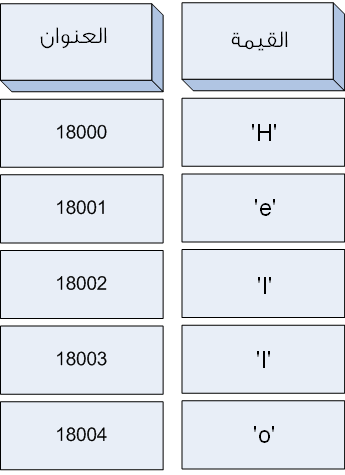
\includegraphics[width=0.4\textwidth]{Chapter_II-4_String-Memory}
\end{figure}

كما نرى فهذا جدول يتكون من 5 خانات في الذاكرة ليمثل الكلمة
'\textenglish{Hello}'.
في المخطط اخترت تمثيل الحروف بين علامتي تنصيص  لأبيّن أنه يتمّ تخزين عدد و ليس حرف. في الحقيقة، دائما في الذاكرة، يتمّ تخزين الأعداد الموافقة لهذه الحروف.

سلسلة المحارف لا تحتوي فقط على الحروف، في الواقع المخطط السابق غير كامل !
السلسلة المحرفيّة
\textbf{تحتوي بالضرورة محرفا خاصّا في النهاية}،
يسمّى "محرف نهاية السلسلة". هذا المحرف يكتب
\InlineCode{\textbackslash 0}.

\begin{question}
  لماذا يجب أن تنتهي السلسلة المحرفيّة بـ\InlineCode{\textbackslash 0} ؟
\end{question}

ببساطة لكي يعرف الحاسوب أين تنتهي السلسلة. المحرف
\InlineCode{\textbackslash 0}
يقول : "توقّف، لا يوجد المزيد لقراءته !".

لذلك، كي نخزن الكلمة
'\textenglish{Hello}'
 لا نحتاج إلى جدول من 5
\InlineCode{char}
و إنما من 6 !\\
في كلّ مرة تقوم فيها بإنشاء سلسلة محرفيّة، يجب عليك أن تفكّر في حجز مكان لمحرف نهاية السلسلة. يجب دائما إضافة خانة لتخزين هذا المحرف
\InlineCode{\textbackslash 0}،
هذا ضروريٌ !

نسيان محرف نهاية السلسلة
\InlineCode{\textbackslash 0}
هو مصدر أخطاء موجعة في لغة
\textenglish{C}.
لهذا فأنا أكرر هذا التحذير أكثر من مرّة.

المخطط التالي هو الأصحّ في تمثيل السلسلة المحرفيّة
'\textenglish{Hello}'
في الذاكرة.

\begin{figure}[H]
	\centering
	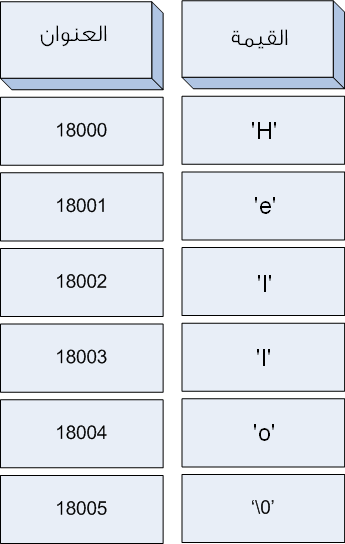
\includegraphics[width=0.4\textwidth]{Chapter_II-4_String-Memory2}
\end{figure}

كما ترى، السلسلة تحوي 6 محارف لا 5، يجب أن يكون الأمر كذلك. السلسلة تنتهي بـ\InlineCode{\textbackslash 0}،
محرف نهاية السلسلة يسمح للحاسوب بمعرفة أين تنتهي السلسلة.

اعتبر المحرف
\InlineCode{\textbackslash 0}
شيئا إيجابيّا لك. بفضله ليس عليك تذكر حجم الجدول الذي خزنته لأنّه يدلّ على مكان توقّف الجدول. يمكنك أن تمرّر جدول
\InlineCode{char}
دون الحاجة إلى استخدام متغيّر يدلّ على حجمه.\\
هذا الأمر صالح فقط للسلاسل المحرفيّة، (أي النوع
\InlineCode{char*}
الذي يمكننا أيضا كتابته على النحو
\InlineCode{char[]}).
بالنسبة للأنواع الأخرى من الجداول، عليك أن تحفظ حجم الجدول في مكان ما.

\subsection{إنشاء و تهيئة سلسلة محرفيّة}

إن أردنا إنشاء جدول
\InlineCode{string}
يحتوي النصّ
'\textenglish{Hello}'،
يمكننا استعمال الطريقة اليدويّة و لكنّها غير فعّالة :

\begin{Csource}
char string[6]; // A table of  6 chars used to store H-e-l-l-o + \0
string[0] = 'H';
string[1] = 'e';
string[2] = 'l';
string[3] = 'l';
string[4] = 'o';
string[5] = '\0';
\end{Csource}

هذه الطريقة تعمل. يمكننا التحقق من ذلك باستعمال
\InlineCode{printf}.

لاستخدام
\InlineCode{printf}
يجب أن نستعمل الرمز
\InlineCode{\%s}
(\textenglish{s}
تعني
\textenglish{String}،
أي "سلسلة محارف" بالإنجليزية). هذه هي الشفرة الكاملة التي تنشئ السلسلة
'\textenglish{Hello}'
في الذاكرة :

\begin{Csource}
#include <stdio.h>
#include <stdlib.h>

int main(int argc, char *argv[])
{
	char string[6]; // A table of 6 chars used to store H-e-l-l-o + \0
	// Initializing the string (writing the letters one by one in the memory)
	string[0] = 'H';
	string[1] = 'e';
	string[2] = 'l';
	string[3] = 'l';
	string[4] = 'o';
	string[5] = '\0';
	// Displaying the string thanks to the %s in the function printf
	printf("%s", string);
	return 0;
}
\end{Csource}

النتيجة :

\begin{Console}
Hello
\end{Console}

تلاحظ أن القيام بتخزين النص حرفا بحرف في الجدول
\InlineCode{string}
أمر متعب للغاية. لتهيئة سلسلة محرفيّة توجد، لحسن الحظ، طريقة أبسط بكثير :

\begin{Csource}
int main(int argc, char *argv[])
{
	char string[] = "Hello"; // The size of the table is automatically calculated
	printf("%s", string);
	return 0;
}
\end{Csource}

\begin{Console}
Hello
\end{Console}

كما تلاحظ في السطر الأول ترى أنني أنشأت متغيّرا من نوع
\InlineCode{char[]}،
كان بإمكاني كتابة
\InlineCode{char*}
أيضاً، النتيجة ستكون نفسها.

عندما تكتب بين علامتي اقتباس (" ") النص الذين تريد تخزينه في الجدول، يقوم الحاسوب بحساب الحجم اللازم. أي أنّه سيحسب عدد الحروف و يضيف 1 من أجل المحرف
\InlineCode{\textbackslash 0}.
يبدأ بعدها في تخزين حروف الكلمة
'\textenglish{Hello}'
واحدا واحدا في الذاكرة و في النهاية يضيف
\InlineCode{\textbackslash 0}
تماما كما فعلنا يديويّا منذ قليل.\\
باختصار، هذا أمر عمليّ أكثر.

و مع ذلك فهناك مشكل : هذا الأمر لا يعمل إلّا مع التهيئة ! لاحقا في الشفرة لا يمكنك كتابة :

\begin{Csource}
string = "Hello";
\end{Csource}

هذه التقنيّة محجوزة للتهيئة فقط. بعد هذا، يجب أن نقوم بالتعديل على المحارف يدويّا في الذاكرة واحداً واحداً كما فعلنا في البداية.

\subsection{إدخال سلسلة محرفيّة عن طريق \texttt{scanf}}

يمكننا حفظ سلسلة محرفّية مُدخَلة من طرف المستخدم عن طريق
\InlineCode{scanf}،
باستخدام الرمز
\InlineCode{\%s}.\\
مشكل وحيد : لا يمكنك معرفة كم محرفا سيقوم المستخدم بإدخاله. إن طلبت منه اسمه الأوّل، فيمكن أن يسمّى
\textenglish{Luc}
(3 محارف)، و لكن من الذي سيضمن أن اسمه لن يكون
\textenglish{Jean-Edouard}
(عدد أكبر بكثير من المحارف) ؟

من أجل هذا، لا يوجد 36 حلّا. يجب إنشاء جدول من
\InlineCode{char}
كبير جدّا، كبير بما يكفي لتخزين الاسم. سنقوم إذن بإنشاء
\InlineCode{char[100]}.
قد تشعر بأنّ هذا إهدار للذاكرة، لكن تذكّر مرّة أخرى بأنّ المكان في الذاكرة ليس الشيء الذي ينقصنا
(كما أنّه توجد برامج تهدر الذاكرة بطريقة أسوء بكثير من هذه !).

\begin{Csource}
int main(int argc, char *argv[])
{
	char firstName[100];
	printf("What's your name ? ");
	scanf("%s", firstName);
	printf("Hello %s, nice to meet you !", firstName);
	return 0;
}
\end{Csource}

\begin{Console}
What's your name ? Mateo21
Hello Mateo21, nice to meet you !
\end{Console}

\section{دوال التعامل مع السلاسل المحرفيّة}

السلاسل المحرفيّة مستعملة بكثرة. فكلّ الكلمات، كلّ النصوص التي تراها على الشاشة هي في الواقع جداول
\InlineCode{char}
في الذاكرة و تعمل كما شرحت لك من قبل.\\
للمساعدة في التعامل مع السلاسل المحرفيّة، توجد المكتبة
\InlineCode{string.h}
التي تحتوي على كم كبير من الدوال التي تقوم بالحسابات على السلاسل المحرفيّة.

لا يمكنني أن أشرحها لك كلّها هنا، سيتطلّب الأمر وقتا طويلا كما أنّها ليست كلّها ضروريّة.\\
سأعلّمك الأساسيّة منها و الّتي ستحتاجها حتما لاحقا.

\subsection{فكّر في تضمين \texttt{string.h}}

حتّى لو بدا لك هذا الأمر بديهيّا، فأنا أفضّل أن أتحدّث عنه مرّة أخرى : بما أنّنا سنستخدم مكتبة جديدة تسمّى
\InlineCode{string.h}،
فيجب أن تضمّنها في أعلى ملفّات
\InlineCode{.c}
حيثما تحتاجها :

\begin{Csource}
#include <string.h>
\end{Csource}

إن لم تقم بهذا فإن المترجم لن يتعرف على الدوال التي سأعرضها لك لأنّه لا يملك نماذجها، و بالتالي فستتوقف الترجمة.\\
باختصار، لا تنس تضمين هذه المكتبة في كلّ مرّة تستخدم فيها دوال التعامل مع النصوص.

\subsection{\texttt{strlen} : حساب طول سلسلة محرفيّة}

\InlineCode{strlen}
تقوم بحساب طول السلسلى المحرفيّة (دون حساب المحرف
\InlineCode{\textbackslash 0}).\\
يحب أن تعطيها معاملا وحيدا : السلسلة المحرفيّة. هذه الدالة تُرجع طول السلسلة.

الآن بما أنّك تعرف مالّذي يعنيه النموذج، سأعطيك نموذج الدوال الّتي أكلّمك عنها. المبرمجون يعتبرونه كـ"دليل استخدام" للدالّة.
هذا نموذج الدالة :

\begin{Csource}
size_t strlen(const char* string);
\end{Csource}

\begin{information}
\InlineCode{size\_t}
هو نوع خاص يدلّ على أنّ الدالة تعيد عددا يمثّل طولا. هو ليس نوعاً قاعديا مثل
\InlineCode{int}،\InlineCode{float}،\InlineCode{char}
و إنما هو نوع  "مُختَرَع". سنتعلم نحن كيف نقوم بإنشاء أنواعنا الخاصة في فصول لاحقة. حاليّا، سنكتفي بتخزين النتيجة التي تعيدها
\InlineCode{strlen}
في متغيّر من نوع
\InlineCode{int}
(سيقوم الحاسوب بالتحويل تلقائيّا من
\InlineCode{size\_t}
إلى
\InlineCode{int}).
يفترض أننا نقوم بتخزين هذه القيمة في متغيّر من نوع
\InlineCode{size\_t}،
لكن عمليّا
\InlineCode{int}
كاف لهذا.
\end{information}

الدالّة تأخد معاملا من نوع
\InlineCode{const char*}.
الـ\InlineCode{const} (التي تعني ثابت، تذكّر) تعني أن الدالة "ستَمتَنِع" عن تغير السلسلة. عندما ترى
\InlineCode{const}،
فستعلم أن المتغيَر لا يتمّ تعديله من طرف الدالّة، بل قراءته فقط.

فلنجرّب الدالّة \InlineCode{strlen}

\begin{Csource}
int main(int argc, char *argv[])
{
	char string[] = "Hello";
	int stringLength = 0;
	// We put the length of string in stringLength
	 stringLength = strlen(string);
	// We display the length of string
	printf("The string %s contains %d characters", string, stringLength);
	return 0;
}
\end{Csource}

\begin{Console}
The string Hello contains 5 characters
\end{Console}

هذه الدالة سهلة الكتابة، يكفي القيام بحلقة على جدول
\InlineCode{char}
حتى تصل إلى المحرف
\InlineCode{\textbackslash 0}.
يوجد عدّاد تتمّ زيادته في كل دورة من الحلقة، و هذا العدّاد يتمّ إعادته في النهاية.

هذا جعلني أريد كتابة شفرة شبيهة بتلك الخاصّة بـ\InlineCode{strlen}. هذا سيمكّنك من أن تفهم جيّدا كيف تعمل هذه الدالّة :

\begin{Csource}
int stringLen(const char* string);
int main(int argc, char *argv[])
{
	char string[] = "Hello";
	int stringLength = 0;
	// We put the length of string in stringLength
	stringLength = stringLen(string);
	// We display the length of string
	printf("The string %s contains %d characters", string, stringLength);
	return 0;
}

int stringLen(const char* string)
{
	int charactersCount = 0;
	char currentCharacter = 0;
	do
	{
    	 	currentCharacter = string[charactersCount];
    	 	charactersCount++;
	}
	while(currentCharacter != '\0'); // We loop while we didn't reach \0
	charactersCount--; // We decrement by 1 in order to not count \0
	return charactersCount;
}
\end{Csource}

هذه الدالة
\InlineCode{stringLen}
تقوم بحلقة على الجدول
\InlineCode{string}.
تقوم في كل مرة بتخزين المحرف الحالي في محرف مُساعد سميناه
\InlineCode{currentCharacter}،
ما إن يكون المحرف الحالي هو
\InlineCode{\textbackslash 0}،
نخرج من الحلقة.

في النهاية نقوم بإنقاص 1 من المجموع، لكي لا نحسب
\InlineCode{\textbackslash 0}.
 قبل نهاية الدالة، نقوم بإرجاع الطول الذي حسبناه أي
\InlineCode{charactersCount}.

\subsection{\texttt{strcpy} : نسخ سلسلة محرفيّة في أخرى}

الدالة
\InlineCode{strcpy}
(و الّتي تعني "\textenglish{String copy}")
تسمح بنسخ سلسلة محرفيّة إلى داخل أخرى.\\
نموذج الدالّة :

\begin{Csource}
char* strcpy(char* stringCopy, const char* stringToCopy);
\end{Csource}

الدالّة تأخذ معاملين :

\begin{itemize}
  \item \InlineCode{stringCopy} : مؤشّر نحو \InlineCode{char*} (جدول \InlineCode{char}). في هذا الجدول يتمّ لصق السلسلة.
  \item \InlineCode{stringToCopy} : مؤشّر نحو جدول آخر من \InlineCode{char}. هذه السلسلة يتمّ نسخها إلى \InlineCode{stringCopy}.
\end{itemize}
الدالّة تعيد مؤشّرا نحو
\InlineCode{stringCopy}،
و هو غير مفيد جدّا. عادة، لا نحفظ ما تعيده هذه الدالّة. فلنجرّبها :
\begin{Csource}
int main(int argc, char *argv[])
{
	char string[] = "Text", copy[100] = {0};
	strcpy(copy, string); // We copy "string" in "copy"
	// If everything is okay, the copy must contain the same thing as string
	printf("string is : %s\n", string);
	printf("copy  is : %s\n", copy);
	return 0;
}
\end{Csource}

\begin{Console}
string is : Text
copy is : Text
\end{Console}

نلاحظ أنّ قيمة
\InlineCode{string}
هي
"\textenglish{Text}".
حتّى الآن، الأمر عاديّ.\\
بالمقابل، نرى أيضا أن المتغيّر
\InlineCode{copy}،
الذي كان فارغا في البداية، قد تمّ ملؤه بمحتوى
\InlineCode{string}.
لقد تمّ فعلا نسخ السلسلة في
\InlineCode{copy}.

\begin{warning}
  تأكّد أن السلسلة
  \InlineCode{copy}
  كبيرة كفاية لاحتواء محتوى
  \InlineCode{string}.
  إن قمت في هذا المثال بتعريف
  \InlineCode{copy[5]}
(و الذي هو غير كاف لأنه لن يبق مكان لـ\InlineCode{\textbackslash 0})،
  الدالّة
  \InlineCode{strcpy}
  "ستخرج عن الذاكرة" و ربّما ستوقف البرنامج عن العمل. تجنّب ذلك، إلّا إذا كنت تريد تعطيل برنامجك.
\end{warning}

النسخ يمكن تمثيله كالتالي :

\begin{figure}[H]
	\centering
	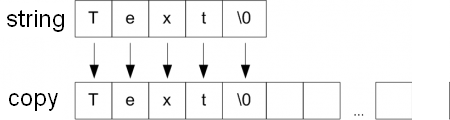
\includegraphics[width=0.6\textwidth]{Chapter_II-4_String-Copy}
\end{figure}
كلّ محرف من
\InlineCode{string}
يتمّ وضعه في
\InlineCode{copy}.\\
السلسلة المحرفيّة
\InlineCode{copy}
تحوي عددا كبيرا من المحارف غير المستعملة، قد لاحظت هذا. أعطيته الحجم 100 من باب الحماية، لكنّ الحجم 6 كان كافيا.
الفائدة من إنشاء جدول أكبر هي أنّه بهذه الطريقة، السلسلة المحرفيّة
\InlineCode{string}
تكون قادرة على احتواء سلاسل أخرى قد تكون أكبر في بقيّة البرنامج.

\subsection{\texttt{strcat} : وصل سلسلتين محرفيّتين}

هذه الدالة تضيف سلسلة محرفيّة إلى نهاية الأخرى. نسمّي هذه العملية بالوصل
(\textenglish{Concatenation}).\\
فلنفرض أن لدينا المتغيّرات التالية :

\begin{itemize}
  \item \InlineCode{string1 = "Hello "}
  \item \InlineCode{string2 = "Mateo21"}
\end{itemize}

إن وصلت
\InlineCode{string1}
في
\InlineCode{string2}
فـ\InlineCode{string2}
ستصبح
\InlineCode{"Hello Mateo21"}.
أمّا بالنسبة لـ\InlineCode{string2}،
فلن تتغيّر و ستكون دائما
\InlineCode{"Mateo21"}.
فقط
\InlineCode{string1}
التي تتغيّر.

هذا تماما ما تفعله
\InlineCode{strcat}، هذا هو نموذجها :

\begin{Csource}
char* strcat(char* string1, const char* string2);
\end{Csource}

كما يمكنك أن ترى،
\InlineCode{string2}
غير قابل للتعديل لأنّه تمّ التصريح عنه كثابت في نموذج الدالّة.\\
الدالّة تعيد مؤشّرا نحو
\InlineCode{string1}،
و مثلما هو الحال مع
\InlineCode{strcpy}،
فهذا لا يصلح لشيء كبير في حالتنا هذه~: يمكننا إذن تجاهل ما تعيده الدالّة.

الدالّة تضيف إلى
\InlineCode{string1}
محتوى
\InlineCode{string2}.
فلنرى هذا عن قرب :

\begin{Csource}
int main(int argc, char *argv[])
{
	char string1[100] = "Hello ", string2[] = "Mateo21";
	strcat(string1, string2); // We concatenate string2 to string1
	// If everything is okay, string1 is equal to "Hello Mateo21"
	 printf("string1 is : %s\n", string1);
	// string2 didn't change :
	printf("string2 is as always : %s\n", string2);
	return 0;
}
\end{Csource}

\begin{Console}
string1 is : Hello Mateo21
string2 is as always : Mateo21
\end{Console}

تأكّد دائما أنّ
\InlineCode{string1}
كبيرة بما فيه الكفاية لكي نستطيع إضافة محتوى
\InlineCode{string2}
إليها، و إلّا فستحدث خروجا عن الذاكرة و قد يتسبب في تعطّل البرنامج.\\
لهذا السبب قمت بتعريف
\InlineCode{string2}
بحجم 100. بينما تركت الحاسوب يحسب حجم
\InlineCode{string1}
تلقائيّا (هذا يعني أنني لم أحدد الحجم) لأنّ هذه السلسلة لا يتمّ تعديلها، فلا حاجة إذن لجعلها أكبر من اللازم.

المخطط التالي يلخّص عمليّة الوصل.

\begin{figure}[H]
	\centering
	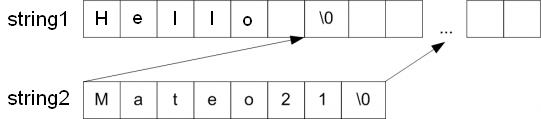
\includegraphics[width=0.6\textwidth]{Chapter_II-4_String-Concatenation}
\end{figure}

الجدول
\InlineCode{string2}
تمّت إضافته إلى نهاية
\InlineCode{string1}
(الذي يحوي 100 خانة).
الـ\InlineCode{\textbackslash 0}
الخاص بـ\InlineCode{string1}
تمّ حذفه (في الواقع تمّ استبداله بـ\textenglish{M} من \textenglish{Mateo21}). في الواقع، لا يجب ترك
\InlineCode{\textbackslash 0}
في وسط سلسلة محرفيّة، و إلّا فسيتمّ "قطعها" في المنتصف ! لا نضع
\InlineCode{\textbackslash 0}
إلّا في نهاية سلسلة محرفيّة، فقط عندما ننهيها.

\subsection{\texttt{strcmp} : مقارنة سلسلتين محرفيّتين}

\InlineCode{strcmp}
تقارن سلسلتين فيما بينهما. هذا هو نموذجها :

\begin{Csource}
int strcmp(const char* string1, const char* string2);
\end{Csource}

المتغيّران
\InlineCode{string1}
و
\InlineCode{string2}
يتمّ مقارنتهما. كما تلاحظ، لا يتمّ تعديل أيّ منهما لأنّه تمّ التصريح عنهما كثوابت.

إنه من الضروري أن نقوم باسترجاع ما تعيده إلينا الدالة. في الواقع، \InlineCode{strcmp} تعيد :

\begin{itemize}
  \item 0 إن كانت السلسلتان متطابقتين.
  \item قيمة أخرى (موجبة أو سالبة) إن كانت السلسلتان مختلفتين.
\end{itemize}

\begin{information}
أعلم أنّه كان من المنطقيّ أكثر أن تعيد الدالّة 1 إن كانت السلسلتين متطابقتين لكي نقول "صحيح" (تذكّر المتغيّرات المنطقيّة). السبب بسيط :
الدالّة تقارن قيم المحارف من كلّ سلسلة واحدا واحدا. إن كانت كلّ المحارف متطابقة فستعيد 0. إن كانت محارف
\InlineCode{string1}
أكبر من محارف
\InlineCode{string2}،
فالدالّة تعيد عددا موجبا. في الحالة المعاكسة تعيد عددا سالبا. عمليّا، نستخدم
\InlineCode{strcmp}
كثيرا للتحقّق من أنّ سلسلتين متطابقتان أم لا.
\end{information}

هذه شفرة التجريب الخاصّة بي :

\begin{Csource}
int main(int argc, char *argv[])
{
	char string1[] = "Test text", string2[] = "Test text";
	if (strcmp(string1, string2) == 0) // If the strings are equal
	{
    		printf("The strings are identical\n");
 	}
	 else
	{
    		printf("The strings are different\n");
	 }
	return 0;
}
\end{Csource}

\begin{Console}
The strings are identical
\end{Console}

بما أنّ السلسلتين متطابقتين، فالدالّة
\InlineCode{strcmp}
أعادت 0.\\
لاحظ أنّه كان بإمكاني تخزين ما أعادته الدالّة في متغيّر من نوع
\InlineCode{int}.
لكنّ ذلك ليس ضروريّا، فيمكننا وضعها مباشرة داخل
\InlineCode{if}
كما فعلت.

ليس لديّ ما أضيفه فيما يتعلّق بهذه الدالّة. هي بسيطة الاستخدام، لكنّ الشيء الوحيد الذي لا يجب نسيانه هو أنّ 0 يعني "متطابق" و أي قيمة أخرى تعني "مختلف". هذا هو مصدر الأخطاء الوحيد هنا.

\subsection{\texttt{strchr} : البحث عن محرف}

الدالّة
\InlineCode{strchr}
تبحث عن محرف في سلسلة محرفيّة. نموذجها :

\begin{Csource}
char* strchr(const char* string, int characterToFind);
\end{Csource}

الدالّة تأخذ معاملين :

\begin{itemize}
  \item \InlineCode{string} : السلسلة التي يتمّ البحث فيها.
  \item \InlineCode{characterToFind} : المحرف الّذي نبحث عنه في السلسلة.
\end{itemize}

\begin{information}
  تلاحظ أنّ
  \InlineCode{characterToFind}
  من نوع
  \InlineCode{int}
  و ليس من نوع
  \InlineCode{char}.
  هذا ليس مشكلا فعلا لأنّه في الواقع المحرف هو عدد. على الرغم من ذلك، نفضّل استخدام
  \InlineCode{char}
  على
  \InlineCode{int}
  لتخزين المحارف في الذاكرة.
\end{information}

الدالة تقوم بإرجاع مؤشر نحو أوّل ظهور للمحرف الذي وجدته في السلسلة، أي أنها ترجع عنوانه في الذاكرة. إن لم تجد شيئا فستعيد
\InlineCode{NULL}.\\
في المثال التالي، سأسترحع هذا المؤشّر في
\InlineCode{restOfString}.

\begin{Csource}
int main(int argc, char *argv[])
{
	char string[] = "Test text", *restOfString = NULL;
	restOfString = strchr(string, 's');
	if (restOfString != NULL) // If we found something
	{
    		printf("This is the rest of the string after the first s:%s", restOfString);
	 }
  return 0;
}
\end{Csource}

\begin{Console}
This is the rest of the string after the first s: st text
\end{Console}

هل فهمت ما حصل ؟ إن الأمر خاصّ قليلا.\\
في الحقيقة، إن
\InlineCode{restOfString}
هو مؤشر مثل
\InlineCode{string}،
إلّا أنّ
\InlineCode{string}
يؤشّر على المحرف الأوّل
(أي \InlineCode{'T'})
بينما
\InlineCode{restOfString}
يؤشّر على أوّل محرف
\InlineCode{'s'}
موجود في
\InlineCode{string}.

المخطّط التالي يوضّح أين يؤشّر كلّ مؤشّر :

\begin{figure}[H]
	\centering
	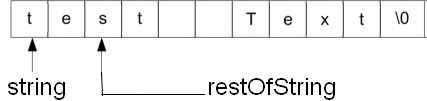
\includegraphics[width=0.5\textwidth]{Chapter_II-4_String-Search}
\end{figure}

عندما أقوم بـ\InlineCode{printf}
لـ\InlineCode{restOfString}،
فمن العاديّ أن يتمّ عرض
"\textenglish{st Text}".
الدالّة
\InlineCode{printf}
تعرض كلّ المحارف التي تلقاها
(\textenglish{s}،\textenglish{t}،\textenglish{T}،\textenglish{e}،\textenglish{x}،\textenglish{t})
حتّى الوصول إلى
\InlineCode{\textbackslash 0}
الذي يعلمها بنهاية السلسلة.

\subsubsection{نسخة مختلفة}

توجد دالّة
\InlineCode{strrchr}
مطابقة تماما لـ\InlineCode{strchr}
باستثناء أنها تعيد مؤشّرا على
\textbf{آخر ظهور للمحرف}
الموجود في السلسلة بدلا من الأوّل.

\subsection{\texttt{strpbrk} : أوّل محرف في القائمة}

هذه الدالّة تشبه كثيرا السابقة. هذه تبحث عن محرف من بين تلك التي تعطيها على شكل سلسلة محرفيّة، بخلاف
\InlineCode{strchr}
التي لا يمكنها البحث عن سوى محرف وحيد في المرّة.

مثلا، إن أعطيناها السلسلة
\InlineCode{"xes"}
و بحثنا في
\InlineCode{"Test text"}،
فالدالّة تعيد مؤشرا نحو أول تكرار لأحد المحارف التي وجدتها.
في هذه الحالة، أوّل محرف من
\InlineCode{"xes"}
الّتي ستجده في
\InlineCode{"Test text"}،
هو الـ\InlineCode{'e'}، إذن
\InlineCode{strpbrk}
تعيد مؤشّرا على
\InlineCode{'e'}.

النموذج :

\begin{Csource}
char* strpbrk(const char* string, const char* charactersToFind);
\end{Csource}

فلنجرّب الدالّة :

\begin{Csource}
int main(int argc, char *argv[])
{
	char *restOfString;
	// We search for the 1st occurrence of x, e or s in "Test text"
	restOfString= strpbrk("Test text", "xes");
	if (restOfString != NULL)
	 {
    		printf("This is the rest of the string starting by the first occurrence of the characters found : %s", restOfString);
	}
	return 0;
}
\end{Csource}

\begin{Console}
This is the rest of the string starting by the first occurrence of the characters found : est text
\end{Console}

في هذا المثال، القيم المراد ارسالها إلى الدالّة مباشرة (بين علامتي اقتباس). لسنا مجبرين على استخدام متغيّر في كلّ المرّات، يمكننا كتابة السلسلة مباشرة.\\
يجب تذكّر هذه القاعدة البسيطة :

\begin{itemize}
  \item إذا استخدمت علامتي الاقتباس \InlineCode{" "}، فهذا يعني \textbf{سلسلة محرفيّة}.
  \item إذا استخدمت علامتي التنصيص \InlineCode{' '}، فهذا يعني \textbf{محرفا}.
\end{itemize}

\subsection{\texttt{strstr} : البحث عن سلسلة محرفيّة في أخرى}

هذه الدالّة تبحث عن أوّل ظهور لسلسلة محرفيّة داخل أخرى.\\
نموذجها :

\begin{Csource}
char* strstr(const char* string, const char* stringToFind);
\end{Csource}

النموذج مشابه لذلك الخاص بـ\InlineCode{strpbrk}،
لكن احذر من الخلط :
\InlineCode{strpbrk}
تبحث عن
\underline{واحد}
من المحارف، بينما
\InlineCode{strstr}
تبحث عن كلّ السلسلة.

مثال :

\begin{Csource}
int main(int argc, char *argv[])
{
	char *restOfString;
	// We search for the 1st occurrence of "text" in "Test text" :
	restOfString = strstr("Test text", "text");
	if (restOfString != NULL)
	 {
    		printf("First occurrence of text in Test text : %s\n", restOfString);
	}
	return 0;
}
\end{Csource}

\begin{Console}
First occurrence of text in Test text : text
\end{Console}

الدالّة
\InlineCode{strstr}
تبحث عن السلسلة
"\textenglish{text}"
في
"\textenglish{Test text}".\\
كغيرها، تعيد مؤشّرا عندما تجد ما تبحث عنه. و تعيد
\InlineCode{NULL}
إن لم تجد شيئا.

حتّى الآن، أنا أقوم بعرض السلسلة عن طريق المؤشّر الّذي تعيده الدالّة. عمليّا، هذا غير مهمّ جدّا. يمكنك فقط القيام بـ\InlineCode{if (result != NULL)}
لمعرفة إن مان البحث قد أعاد أيّ شيء، و تُظهر "النصّ الذي تبحث عنه قد تمّ العثور عليه".

\subsection{\texttt{sprintf} : الكتابة في سلسلة محرفيّة}

\begin{information}
  هذه الدالّة موجودة في
  \InlineCode{stdio.h}
  بخلاف الدوال التي درسناها إلى حدّ الآن، و التي كانت في
  \InlineCode{string.h}
\end{information}

هذا الاسم يذكّرك بشيء ما. هذه الدالّة مشابهة إلى حدّ كبير لـ\InlineCode{printf}
التي تعرفها، و لكن بدل الكتابة على الشاشة،
\InlineCode{sprintf}
تكتب في \dots سلسلة محرفيّة ! و من هذا اسمها الذي يبدأ بـ"\textenglish{s}" من "\textenglish{string}" (سلسلة محرفيّة بالإنجليزيّة).

إنّها دالّة عمليّة جدّا لتنسيق سلسلة محرفيّة. مثال صغير :

\begin{Csource}
#include <stdio.h>
#include <stdlib.h>
int main(int argc, char *argv[])
{
	char string[100];
	int age = 15;
	// We write "You have 15 years" in string
	sprintf(string, "You have %d years !", age);
	// We display string to check its content
	printf("%s", string);
	return 0;
}
\end{Csource}

\begin{Console}
You have 15 years !
\end{Console}

تُستخدم بنفس طريقة
\InlineCode{printf}
باستثناء أنّه يجب إعطائها كمعامل أوّل مؤشّرا نحو السلسلة التي يجب أن تستقبل النصّ.

في هذا المثال، أكتب في
\InlineCode{string}
"\textenglish{You have \%d years}"،
حيث يتمّ استبدال
\InlineCode{\%d}
بمحتوى المتغيّر
\InlineCode{age}.
كلّ قواعد
\InlineCode{printf}
تطبّق، يمكنك إذا أردت أم تضع
\InlineCode{\%s}
لإدراج سلاسل أخرى داخل سلسلتك~!

كالعادة، تأكّد أن سلسلتك كبيرة كفاية لاحتواء النصّ الذي سترسله لها
\InlineCode{sprintf}.
و إلّا، فقد يحدث تجاوز في الذاكرة و بالتالّي تعطّل برنامجك.

\section*{ملخّص}

\begin{itemize}
  \item الحاسوب لا يجيد التعامل مع النصوص، هو لا يعرف إلّا الأعداد. لإصلاح هذا المشكل، تمّ ربط كلّ حرف بعدد موافق له في جدول يسمّى
  \textbf{جدول \textenglish{ASCII}}.
  \item النوع \InlineCode{char} يستخدم لتخزين حرف واحد. يخزّن في الحقيقة عددا، لكنّ هذا العدد تتمّ ترجمته إلى حرف من طرف الحاسوب أثناء العرض.
  \item لإنشاء كلمة أو جملة، علينا بناء
  \textbf{سلسلة محرفيّة}.
  من أجل هذا، نستخدم
  \textbf{جدول \texttt{char}}.
  \item كلّ سلسلة محرفيّة تنتهي بمحرف خاصّ يكتب
  \InlineCode{\textbackslash 0}
  يعني "نهاية السلسلة".
  \item توجد الكثير من الدوال الجاهزة للتعامل مع السلاسل المحرفيّة في
  \textbf{المكتبة \textenglish{string}}.
  يجب تضمين
  \InlineCode{string.h}
  لاستخدامها.
\end{itemize}
